% Manuscript source.
\documentclass[11pt]{article}
\pagestyle{plain}
\usepackage[margin=1in]{geometry}
\usepackage[T1]{fontenc}
\usepackage[utf8]{inputenc}
\usepackage{lmodern}
\input{glyphtounicode}
\pdfgentounicode=1
\usepackage{amsmath,amssymb,amsthm}
\usepackage{booktabs,array}
\usepackage{graphicx}
\usepackage{enumitem}
\usepackage[title]{appendix}
\usepackage{fvextra}
\usepackage{newunicodechar}
\usepackage{xcolor}
\usepackage[hyphens]{url}
\usepackage{hyperref}
\hypersetup{colorlinks=true,linkcolor=blue,citecolor=blue,urlcolor=blue,
  pdfauthor={P. Graham},
  pdftitle={The three-color Ramsey number of the 10-vertex path}}

% Unicode characters in the Lean listings.
\newunicodechar{ℕ}{\ensuremath{\mathbb{N}}}
\newunicodechar{∃}{\ensuremath{\exists}}
\newunicodechar{∀}{\ensuremath{\forall}}
\newunicodechar{∧}{\ensuremath{\wedge}}
\newunicodechar{→}{\ensuremath{\to}}
\newunicodechar{⟨}{\ensuremath{\langle}}
\newunicodechar{⟩}{\ensuremath{\rangle}}
\newunicodechar{≤}{\ensuremath{\le}}
\newunicodechar{∈}{\ensuremath{\in}}
\newunicodechar{¬}{\ensuremath{\neg}}
\fvset{fontsize=\small,breaklines=true}

\newtheorem{theorem}{Theorem}[section]
\newtheorem{lemma}[theorem]{Lemma}
\newtheorem{proposition}[theorem]{Proposition}
\newtheorem{corollary}[theorem]{Corollary}
\newtheorem{conjecture}[theorem]{Conjecture}
\theoremstyle{definition}
\newtheorem{definition}[theorem]{Definition}
\theoremstyle{remark}
\newtheorem{remark}[theorem]{Remark}

\newcommand{\lex}{\le_{\mathrm{lex}}}
\newcommand{\R}{R_3}
\setlength{\emergencystretch}{3em}

\title{The three-color Ramsey number of the 10-vertex path}
\author{P. Graham\\ \small\url{https://orcid.org/0009-0007-8493-1505}}
\date{October 24, 2026}

\begin{document}
\maketitle
\begin{abstract}
Writing $P_n$ for the path on $n$ vertices and $R_3(P_n)=R(P_n,P_n,P_n)$
for its three-color Ramsey number, Gyárfás, Ruszinkó, Sárközy and
Szemerédi proved $R_3(P_n)=2n-2+(n\bmod2)$ for all sufficiently large $n$
\cite[author manuscript, July 9, 2012, Theorem~1]{GRSS07}.
Dybizbański, Dzido and Radziszowski (DDR) established $R_3(P_8)=14$ and
$R_3(P_9)=17$ \cite[arXiv:1207.5851v3, Theorems~10 and~8 with Section~2]{DDR16},
completing the cases $n\le9$ recorded by Radziszowski's survey
\cite[revision~18, p.~65, Section~6.4.1(c)]{Rad26}.
We prove the next case, $R_3(P_{10})=18$: every three-coloring of the
edges of $K_{18}$ contains a monochromatic ten-vertex path, while a coloring
of $K_{17}$ contains none. The new bound is the upper bound $18$; the lower
bound uses the even-case $K_4$ blow-up in
\cite[Section~1.1, after Theorem~1]{GRSS07} and \cite[Section~2]{DDR16}.
This is the ten-vertex case of Conjecture~2 in the cited DDR version,
which credits Faudree and Schelp's 1975 suggestion.
Boolean satisfiability refutations prove the upper bound. Lean checks the
full certificate proof using trusted native evaluation; the default Lake
build alone is conditional.
\end{abstract}

\noindent The proofs, the Lean formalization, the search code, the certificate checkers and the text were produced by AI models (from OpenAI and Anthropic), working under the author's direction.

\section{The result}
For graphs $G_1,G_2,G_3$, the Ramsey number $R(G_1,G_2,G_3)$ is the least
$N$ such that every coloring of the edges of $K_N$ with colors $1,2,3$
contains, for some $i$, a copy of $G_i$ all of whose edges have color $i$.
We write $\R(G)=R(G,G,G)$, and $P_n$ for the path on $n$ vertices (with
$n-1$ edges). Paths are not required to be induced.

\begin{theorem}\label{thm:main}
$\R(P_{10})=18$. That is, every coloring of the edges of $K_{18}$ with
three colors contains a monochromatic path on $10$ vertices, and some
$3$-coloring of the edges of $K_{17}$ contains none.
\end{theorem}

The advance is the upper bound $\R(P_{10})\le18$.
Gyárfás, Ruszinkó, Sárközy and Szemerédi proved
$\R(P_n)=2n-2+(n\bmod2)$ for all sufficiently large $n$
\cite[author manuscript, July 9, 2012, Theorem~1]{GRSS07}, with its corrigendum.
Dybizbański, Dzido and Radziszowski proved $\R(P_8)=14$
(Theorem~10) and $\R(P_9)\le17$ (Theorem~8), which with their Section~2
lower bound gives $\R(P_9)=17$ \cite[arXiv:1207.5851v3]{DDR16}.
Radziszowski's survey \cite[revision~18, p.~65, Sections~6.4 and~6.4.1(c)]{Rad26}
records the formula through $n=9$ and $P_{10}$ as the first open case.
Our $K_{17}$ lower bound is the even-case blow-up in
\cite[Section~1.1, after Theorem~1]{GRSS07}, also given in
\cite[arXiv:1207.5851v3, Section~2]{DDR16}.
The latter attributes Conjecture~2's suggestion to Faudree and Schelp
(1975), quoting ``they feel''; its closing remarks say,
``We did not complete these proofs'', referring to $P_{10}$ and $P_{11}$.
This paper settles $n=10$ of Conjecture~\ref{conj:FS}; the general
conjecture remains open.

Heule, Kullmann, Wieringa and Biere's cube-and-conquer
\cite[author manuscript, Section~3, Overview]{HKWB12} ``partitions a formula
into many subformulas''.
We use the verified LRAT checker from the \texttt{bv\_decide} work of
Böving et al.\ \cite[version of record, introduction, contributions, and
Section~4.4]{BBC+25}, which lists an ``LRAT UNSAT proof checker''.
Szeider's streaming tool \texttt{lrat-catcher}
\cite[arXiv:2607.00815v2, abstract]{Sze26} ``turns a certificate into a Lean
theorem'' using Lean core's verified checker.
Our certificate import uses the same checker, with its own compact
certificate encoding (Appendix~\ref{sec:certs}).

For the verification method, Kirchweger, Manrique and Szeider
\cite[IJCAR 2026, abstract]{KMS26} describe ``a unified, machine-checked
verification pipeline'' for graph generation.

Related computations include Heule, Kullmann and Marek's Boolean
Pythagorean triples proof \cite[author preprint, Theorem~1]{HKM16},
Codish, Frank, Itzhakov and Miller's ``$R(4,3,3)=30$''
\cite[author preprint, abstract]{CFIM16}, and Heule and Scheucher's
``An empty hexagon in every set of 30 points'' \cite[TACAS 2024, title]{HS24},
with Subercaseaux et al.'s ``Formal verification of the empty hexagon
number'' \cite[ITP 2024, title]{SNG+24}.
Wesley's Theorems~3 and~4 give
$R(C_3,C_6,C_6)=R(C_5,C_6,C_6)=15$ \cite[arXiv:2509.03784v1]{Wes25}.
Galindez reports ``$R(C_{10},C_{10},C_{10})\le26$''
\cite[Zenodo record title]{Gal26}, using cube-and-conquer and
Kirchweger--Szeider's ``SAT modulo symmetries'' \cite[TOCL 2024, title]{KS24};
Shao, Jiang, Xu and Wang provide the ``reproduction package:
$R(C_4,C_6,C_8)=12$'' \cite[Zenodo record title]{SJXW26}.
Posted work also includes Leo-Y-Zhang's ``CycleRamsey'' \cite[repository title]{Zha26}
and Zhang's $k$-color tree-bound corollary $R_k(T)\le k(n-2)+2$ for trees on $n\ge2$
vertices \cite[pinned README, Ramsey corollary]{ZhJ26}, from the
GPT-6 Astra proof packaged by Adamczewski; it gives $\R(P_{10})\le26$.
Allen et al. consider ``Ramsey-type problems for paths and cycles''
\cite[arXiv:2607.03243v1, title]{ABC+26}.

For ``Ramsey numbers for paths'', see Dzido \cite[title]{Dzi05} and
Dzido--Fidytek \cite[title]{DF09}; Omidi--Raeisi treat ``paths versus
cycles'' \cite[title]{OR11}, and Maherani et al. give mixed-path cases
\cite[arXiv:1207.3771v1, Theorem~1.1]{MORS15}.
Earlier cycle work includes Benevides--Skokan's ``even cycles''
\cite[title]{BS09}, Figaj--Łuczak's ``long even cycles'' \cite[title]{FL07},
and Letzter's ``connected matchings method'' \cite[title]{Let22}.
Small-case credit to Irving, Yang--Rowlinson and Yang
\cite{Irv74,YR94,YR92,Yan95} follows the survey
\cite[revision~18, p.~65, Section~6.4.1(c)]{Rad26}.
The extremal comparison credits Erdős--Gallai's ``maximal paths and
circuits'' \cite[title]{EG59} and the Faudree--Schelp theorem
\cite{FS75} as recalled in DDR \cite[arXiv:1207.5851v3, Theorem~4]{DDR16}.
Kopylov's ``Maximal paths and cycles in a graph'' \cite[title]{Kop77}
gives related context.
We use de~Moura and Ullrich's Lean~4 \cite{MU21} and the mathlib
Community's library \cite{Mathlib20}.
The separate checks use Wetzler, Heule and Hunt's \texttt{drat-trim}
\cite[title]{WHH14} for conversion to Cruz-Filipe et al.'s LRAT format
\cite[abstract]{CHH+17}, and Tan, Heule and Myreen's \texttt{cake\_lpr}
\cite[title]{THM21} for checking.

\section{Proof overview}
The difficult step is obtaining a tractable case split without losing
a coloring: fixing a guaranteed path and imposing symmetry constraints
must be jointly sound, and discarded branches leave a coverage obligation.
A lexicographic minimum and a separate cover refutation discharge these
obligations. The earlier obstruction is explicit in the closing remarks
of Dybizbański, Dzido and Radziszowski~\cite[arXiv:1207.5851v3, Section~5]{DDR16}:
``the complexity of case analysis appears to be quite harder''.
The reduction starts with a monochromatic $P_9$, as in the bound
of Dybizbański, Dzido and Radziszowski, Theorem~8 of the version
cited above. Here that bound is re-derived by smaller Boolean satisfiability (SAT)
refutations, starting with $P_3$ on $K_5$ and ending with $P_9$ on
$K_{17}$. Each refutation fixes only the path guaranteed by the preceding
one. The construction in Figure~\ref{fig:lower} supplies the matching
lower bound; Appendix~\ref{sec:lower} gives its proof.

\begin{figure}[ht]
\centering
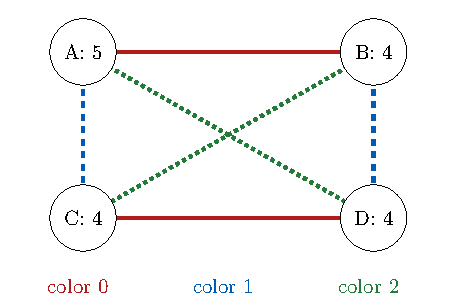
\includegraphics[width=.42\textwidth]{../data/lower-bound.pdf}
\caption{The $K_{17}$ coloring, compressed into four parts. Each line
represents all edges between its parts; all edges within a part have
color~0. In each color, the two label classes have sizes 9 and 8.}
\label{fig:lower}
\end{figure}

A Boolean literal is a variable or its negation; a clause is a
disjunction of literals.
Each logged path clause is rebuilt in Lean from its color and distinct
vertices. Refuting this subset suffices: a coloring without a monochromatic
path would satisfy every path clause, hence also the logged subset.
Cubes are conjunctions of literals fixing edge colors. A separate cover
refutation proves that every model satisfies at least one listed cube;
each cube has its own refutation. Lemma~\ref{lem:cover} joins these facts.
Appendices~\ref{sec:encoding}--\ref{sec:cnc} give the encoding, the
reductions and this complete dependency chain.

\section{What is checked and trusted}
In namespace \texttt{R3P10}, the unconditional theorem is
\texttt{R3\_P10\_eq\_18 : ramsey3Path 10 = 18}.
Here \texttt{Col n} is \texttt{Sym2 (Fin n) → Fin 3}: colors on unordered
vertex pairs. Diagonal values are unused and arbitrary; colors $0,1,2$
replace $1,2,3$. The predicate \texttt{HasMonoPath n m X} means that there
exist a color and an injective map from $m$ vertices to $n$ vertices whose
consecutive pairs have that color. It requires no condition on other
pairs, so it means our non-induced $P_m$, with $m$ vertices, not edges.
The definition \texttt{ramsey3Path m} is the infimum in the natural numbers
of the $n$ for which every \texttt{Col n} satisfies that predicate.
The proof establishes membership at $18$ and a countercoloring at $17$;
restriction of that coloring excludes every smaller $n$. Thus this
infimum is precisely the Ramsey number in Theorem~\ref{thm:main}, with
no remaining certificate hypotheses.

Lean proves the lower bound, symmetry reductions, encoding soundness and
assembly of refutations. Its verified LRAT checker checks a line-indexed
format of propositional refutations. The final theorem's axioms are
\texttt{propext}, \texttt{Classical.choice}, \texttt{Quot.sound},
\texttt{Lean.ofReduceBool} and \texttt{Lean.trustCompiler}.
The last two support native evaluation of certificate checks, list lengths
and the parsed-formula comparison. The proof trusts Lean's kernel,
compiler and imported compiled modules; rebuilding the certificate modules
avoids trusting previously built copies. The SAT solver, converter and
external checkers are outside this trusted base. Literature attributions,
historical timings and reports of separate checker executions are outside
Lean. Appendix~\ref{sec:lean} gives the declarations and dependency details.

From the accompanying folder, \texttt{cd lean},
\texttt{lake exe cache get}, then \texttt{lake build} check the
reduction, lower bound and conditional theorem, not the unconditional
value. The full command \texttt{python3 checks/check.py full}
regenerates and checks every certificate and builds \texttt{R3P10Final}.
Installing the archived certificates~\cite{Gra26} first avoids repeating
the search. Quick mode checks a sample and cannot replace the full check.
See \path{COMPLETION.md} for the completed full check and
\path{checks/README.md} and \path{lean/README.md} for requirements,
commands and independent checks. The proof is computer-assisted and has not been reviewed by human experts.

\clearpage
\begin{appendices}
\section{The conjecture}
The general conjecture is Conjecture~2 of Dybizbański, Dzido and
Radziszowski~\cite[arXiv:1207.5851v3, Section~2]{DDR16}; its ten-vertex
case is proved here.
\begin{conjecture}[suggested by Faudree--Schelp~\cite{FS75}; stated as a conjecture in~\cite{DDR16}; see~\cite{Rad26}]\label{conj:FS}
For all $n\ge1$, $\R(P_n)=2n-2+(n\bmod 2)$.
\end{conjecture}

\section{The lower bound}\label{sec:lower}

Partition $\{0,\dots,16\}$ into $A=\{0,\dots,4\}$, $B=\{5,\dots,8\}$,
$C=\{9,\dots,12\}$ and $D=\{13,\dots,16\}$. Color an edge with color $0$
if both ends lie in $A\cup B$ or both lie in $C\cup D$; with color $1$ if
it joins $A$ to $C$ or $B$ to $D$; and with color $2$ if it joins $A$ to
$D$ or $B$ to $C$. This is the blow-up of the factorization of $K_4$ into
the matchings $\{AB,CD\}$, $\{AC,BD\}$, $\{AD,BC\}$, with the edges inside
the parts given color $0$. For this construction, Gyárfás, Ruszinkó, Sárközy and Szemerédi
\cite[author manuscript, July 9, 2012, Section~1.1, paragraph following
Theorem~1]{GRSS07} write: ``One type comes from a `blow-up' of a
factorization of $K_4$.'' The odd and even part sizes are specified there;
see also Dybizbański, Dzido and Radziszowski~\cite[arXiv:1207.5851v3,
Section~2, paragraph following Conjecture~2]{DDR16}.

\begin{proposition}\label{prop:lower}
This coloring of $K_{17}$ has no monochromatic $P_{10}$. Hence
$\R(P_{10})\ge 18$.
\end{proposition}

\begin{proof}
Each color has two label classes: $A\cup B$ and $C\cup D$ for color $0$,
$A\cup C$ and $B\cup D$ for color $1$, $A\cup D$ and $B\cup C$ for color
$2$, of sizes $9$ and $8$ in each case. The edge invariant is that every
edge of a color lies inside one of that color's two label classes; no edge
of that color joins them. So every connected piece of a color class lies
inside one label class and has at most $9$ vertices, and a monochromatic
path, being connected, has at most $9$ vertices.
\end{proof}

In Lean the coloring is written out edge by edge, and the argument is a
general lemma (for all $n$ and $m$: if each color has a labeling of the
vertices that is constant along edges of that color and whose classes have
fewer than $m$ vertices, there is no monochromatic $P_m$) together with two
finite facts decided by the kernel's own reduction (\texttt{decide
+kernel}), without native evaluation.

\section{The encoding}\label{sec:encoding}

For the upper bound, suppose a coloring of $K_{18}$ has no monochromatic
$P_{10}$. Relabel vertices and colors so that $0,1,\ldots,8$ is a path
of color~0. Among colorings reachable by permutations that preserve this
path, take a lexicographically least one. It satisfies every imposed
symmetry inequality simultaneously (Lemmas~\ref{lem:fix}
and~\ref{lem:lex}). The chosen symmetries need not include every
permutation preserving the path.

A Boolean literal is a variable or its negation; a clause is a
disjunction of literals. A model assigns truth values satisfying every
clause; a refutation certifies that no such assignment exists.
The SAT variables specify one color per edge, with auxiliary variables
expressing the symmetry inequalities. A path clause excludes a specified
monochromatic $P_{10}$. Rather than list all paths, the solver logs the
path clauses it uses. Each is independently recognized as a path clause
and rebuilt in Lean from its color and distinct vertices. Refuting this
subset suffices: a coloring without a monochromatic path would satisfy
every path clause, hence also the logged subset. The solver's path-finding
procedure therefore need not be trusted for completeness.

The remaining formula is divided into cubes, conjunctions of literals
fixing edge colors. A separate cover refutation proves that every model
satisfies at least one listed cube; each cube has its own refutation.
Lemma~\ref{lem:cover} joins these facts, contradicting the assumed
coloring. The same argument establishes each smaller bound used to fix a
path. Appendices~\ref{sec:encoding}--\ref{sec:cnc} give the encoding,
the reductions and this complete dependency chain.


Throughout, a \emph{coloring} of $K_n$ is a map $X$ from the edges to
$\{0,1,2\}$, and it is \emph{good} (for $m$) if it has no monochromatic
$P_m$. We order the edges $\{i,j\}$, $i<j$, row by row:
$\{0,1\},\{0,2\},\dots,\{0,n-1\},\{1,2\},\dots,\{n-2,n-1\}$, and number
them $e=0,1,\dots,\binom n2-1$ in this order.

\subsection{Variables and the coloring clauses}
The variable $x_{e,c}=3e+c+1$ means ``edge $e$ has color $c$''.
An unordered pair in the edge subscript denotes its number in the preceding edge order. For each
edge there is one clause $x_{e,0}\vee x_{e,1}\vee x_{e,2}$ and three
clauses $\neg x_{e,c}\vee\neg x_{e,d}$, $c<d$, so that models correspond to
colorings. For a color $c$ and distinct vertices $p_0,\dots,p_{m-1}$, the
\emph{path clause}
\[
\bigvee_{i=0}^{m-2}\neg x_{\{p_i,p_{i+1}\},c}
\]
says that this path is not monochromatic in color $c$. A coloring is good
exactly when its assignment satisfies every path clause. The path clauses
are not written into the formula in advance; they are generated during the
search (Section~\ref{sec:prop}).

\subsection{The fixed path}
Vertex permutations $\pi\in S_n$ and color permutations $\sigma\in S_3$ act
on colorings by $(g\cdot X)(\{\pi a,\pi b\})=\sigma(X(\{a,b\}))$ for
$g=(\pi,\sigma)$. They map good colorings to good colorings.

Here ``good'' means having no monochromatic $P_m$, for the same $m$
as in the preceding encoding. The following lemma fixes only path edges.

\begin{lemma}[fixed path]\label{lem:fix}
Let $k\le n$ and suppose every $3$-coloring of $K_n$ contains a
monochromatic $P_k$. Then every good coloring of $K_n$ is equivalent under
$S_n\times S_3$ to a good coloring $X$ with $X(\{t,t+1\})=0$ for
$0\le t\le k-2$.
\end{lemma}

\begin{proof}
Take a monochromatic path $v_0,\dots,v_{k-1}$ in color $c$; apply a vertex
permutation sending $v_t$ to $t$ and the transposition of colors $c$ and
$0$.
\end{proof}

The formula for the rung ``$P_m$ on $K_n$ with a fixed $P_k$'' contains
the $k-1$ unit clauses $x_{\{t,t+1\},0}$. Only the path edges are
constrained; the chords of the fixed path are free.

\subsection{Lex-leader constraints}
Compare colorings by the lexicographic order $\lex$ of their color vectors
$(X(e))_{e}$ in edge order, with $0<1<2$. Let $\Gamma$ be a list of
generators $g=(\pi,\sigma)$. With a fixed $P_k$ on $0,\dots,k-1$ and
$W=\{k,\dots,n-1\}$, $\Gamma$ consists of the transpositions of pairs of
vertices of $W$ (in lexicographic order), the reversal $t\mapsto k-1-t$ of
$\{0,\dots,k-1\}$, and the color transposition $1\leftrightarrow2$. On the
first rung, $K_5$, nothing is fixed and $\Gamma$ consists of all vertex
transpositions and the color transpositions $0\leftrightarrow1$ and
$1\leftrightarrow2$.

In the following lemma, goodness still refers to $P_m$ and $\Gamma$ is
the preceding list of path-preserving vertex and color permutations.

\begin{lemma}[lex-leader]\label{lem:lex}
Let $S$ be the set of good colorings with color $0$ on the fixed path.
Each $g\in\Gamma$ maps $S$ to itself. Consequently, if $S$ is nonempty it
contains a coloring $X^*$ with $X^*\lex g\cdot X^*$ for every
$g\in\Gamma$.
\end{lemma}

\begin{proof}
When a path is fixed, each vertex permutation in $\Gamma$ maps the
path's edge set to itself and each color permutation in $\Gamma$ fixes
color $0$, so $\Gamma$ preserves the fixed path; every $g$ preserves
goodness. (With nothing fixed, $S$ is the set of all good colorings.) Take $X^*$ to be the $\lex$-least coloring reachable from a
member of $S$ by finitely many moves from $\Gamma$; it lies in $S$, and
$g\cdot X^*$ is reachable too, so $X^*\lex g\cdot X^*$.
\end{proof}

The point of Lemma~\ref{lem:lex} is that the lex-leader constraints for
\emph{every} generator hold simultaneously for one coloring that also has
the fixed path; the two reductions are therefore jointly sound. The
generators do not need to generate the full stabilizer of the fixed path:
a weaker set of constraints only leaves more symmetry in the search.

The constraint $X\lex g\cdot X$ is encoded in the standard
way~\cite[technical report TR-1996-012, Section~3,
Proposition~3.1 and the following auxiliary-variable clauses]{CGLR96}. The clauses below adapt that Boolean-variable construction to three colors. The positions compared are the edges $f$ in edge order,
except those with $\pi^{-1}(f)=f$ and $\sigma$ the identity (where
$X(f)=(g\cdot X)(f)$ identically). For the $j$-th compared position $f_j$,
let $Y_j=\sigma(X(\pi^{-1}f_j))$ be the color of $g\cdot X$ there, and let
$q_j$ be an auxiliary variable meaning ``$X$ and $g\cdot X$ agree on the
first $j$ compared positions'' ($q_0$ is true and omitted). The clauses
are, for colors $a,b$:
\begin{align*}
&q_{j-1}\to\neg\bigl(X(f_j)=a\wedge Y_j=b\bigr)\quad(a>b), &
&q_{j-1}\wedge X(f_j)=a\wedge Y_j=a\to q_j,\\
&q_j\to q_{j-1}, &
&q_j\wedge X(f_j)=a\to Y_j=a.
\end{align*}
Under the intended meaning of the $q_j$, every clause holds exactly when
$X\lex g\cdot X$. For $K_{18}$ with a fixed $P_9$ there are $38$
generators ($36$ transpositions of the nine vertices of $W$, the reversal,
and the color swap), and the base formula has $1{,}868$ variables ($459$
color variables and $1{,}409$ auxiliaries) and $14{,}672$ clauses.

\subsection{Path clauses generated during the search}\label{sec:prop}
The solver is CaDiCaL~\cite{BFF+24} with an external propagator attached
through the IPASIR-UP interface~\cite{FNP+23,FNP+24}. The propagator
follows the assignment of the color variables. Whenever an edge receives a
color $c$, it searches for paths on $m$ vertices through that edge, in the
graph of edges not yet excluded from color $c$, all of whose edges except
at most one are already known to have color $c$. If all edges are known,
it reports the path clause as a conflict; if exactly one is unknown, it
sets that edge to ``not $c$'' with the path clause as the reason. When the
solver reaches a complete assignment, the propagator searches it
exhaustively for a monochromatic $P_m$ and, if it finds one, rejects the
assignment with that path clause. Every clause handed to the solver is a
path clause and is written to a log.

The refuted formula is therefore the base formula plus the logged path
clauses (plus a cube's unit clauses), a subset of the formula with
\emph{all} path clauses. A refutation of the subset refutes the full
formula; nothing about the completeness of the propagator is needed.
Conversely, a satisfying assignment is accepted only after the exhaustive
search, and every coloring the method reports is rechecked by a separate
program.

\section{The ladder}\label{sec:ladder}

The rung ``$P_m$ on $K_n$, fixing $P_k$'' is the formula of
Section~\ref{sec:encoding} with the fixed path on $0,\dots,k-1$, together
with all path clauses for $P_m$. If it is unsatisfiable and every
$3$-coloring of $K_n$ contains a monochromatic $P_k$, then by
Lemmas~\ref{lem:fix} and~\ref{lem:lex} every $3$-coloring of $K_n$
contains a monochromatic $P_m$. Every $3$-coloring of a larger complete
graph then does too, by restriction.

Table~\ref{tab:ladder} lists the rungs. The first fixes nothing; each later
rung fixes the path guaranteed by the rung before it. A DRAT proof is a
clause-addition and deletion refutation, converted to the line-indexed LRAT
format for checking. Each rung up to
$P_9$ on $K_{17}$ is solved as one formula, with a DRAT proof. The rungs
establish the upper bounds $\R(P_m)\le n$ for $m=3,\dots,9$; the top
rung, $P_{10}$ on $K_{18}$, uses $\R(P_9)\le17$ as established by the
rung below it. The earlier $P_9$ bound is Theorem~8 of Dybizbański,
Dzido and Radziszowski~\cite[arXiv:1207.5851v3, Section~4]{DDR16}.

\begin{table}[ht]
\centering
\begin{tabular}{@{}lrrrr@{}}
\toprule
Rung & fixed path & variables & base clauses & logged path clauses\\
\midrule
$P_3$ on $K_5$ & none & 110 & 828 & 11\\
$P_4$ on $K_6$ & $P_3$ & 92 & 527 & 31\\
$P_5$ on $K_9$ & $P_4$ & 308 & 2{,}135 & 185\\
$P_6$ on $K_{10}$ & $P_5$ & 368 & 2{,}502 & 1{,}683\\
$P_7$ on $K_{13}$ & $P_6$ & 828 & 6{,}234 & 10{,}094\\
$P_8$ on $K_{14}$ & $P_7$ & 928 & 6{,}897 & 60{,}734\\
$P_9$ on $K_{17}$ & $P_8$ & 1{,}720 & 13{,}633 & 520{,}545\\
$P_{10}$ on $K_{18}$ & $P_9$ & 1{,}868 & 14{,}672 & (per cube)\\
\bottomrule
\end{tabular}
\medskip
\caption{The ladder. Each rung from $P_3$ to $P_9$ is refuted as a whole;
the largest takes a few CPU-minutes. The $K_{18}$ rung is split into cubes
(Section~\ref{sec:cnc}).}\label{tab:ladder}
\end{table}

The same code also finds colorings where they exist. For example it finds
good colorings for $P_5$ on $K_8$, $P_6$ on $K_9$, $P_7$ on $K_{12}$ and
$P_8$ on $K_{13}$, and, with no fixed path, a coloring of $K_{16}$ with no
monochromatic $P_9$; each was confirmed by a separate exhaustive path
search.

\section{Cube and conquer on \texorpdfstring{$K_{18}$}{K18}}\label{sec:cnc}
This section constructs the split, proves its coverage and joins the refutations.

\subsection{The cubes}
A cube is a conjunction of literals fixing the colors of some edges.
Unit propagation forces the last unassigned literal of a clause when
all its other literals are false. The
cubes were produced by the solver itself, with the propagator attached.
Walking the edges in edge order, at each edge it assumes each color in
turn and runs unit propagation (including the path propagator); colors
leading to a conflict are dropped, an edge with a single surviving color
is fixed without counting as a split, and the walk stops after $10$ edges
with at least two surviving colors. This produced $15{,}316$ cubes of
$11$ to $20$ literals, and $18$ path clauses learned during generation.

Sixteen of these cubes, each with $11$ literals, are listed in
\path{data/k18/split/parents.txt}. Each was split once more in the same way, by four further split
edges, into $41$ children, $656$ in all ($144$ more path clauses were
learned during this split). The final list consists of the $15{,}300$
remaining first-level cubes and the $656$ children: $15{,}956$ cubes.

\subsection{The reduction chain}\label{sec:chain}
Suppose a $3$-coloring $X$ of $K_{18}$ has no monochromatic $P_{10}$. Since
$\R(P_9)\le17$ (the top rung of the ladder, itself resting on the rungs
below it, down to $P_3$ on $K_5$, which fixes nothing), $X$ contains a
monochromatic $P_9$. By Lemma~\ref{lem:fix} a vertex permutation and a
color permutation carry $X$ to a good coloring with color $0$ on the path
$0,1,\dots,8$, and by Lemma~\ref{lem:lex} its orbit under the generators
contains a good coloring $X^*$ that keeps the fixed path and satisfies
every lex-leader inequality. With the auxiliaries set to their meaning,
$X^*$ satisfies the base formula and every path clause. By the cover
certificate, $X^*$ satisfies some cube of the final list (otherwise it
would satisfy the cover formula), and that cube's formula is unsatisfiable
by its own certificate: a contradiction. In Lean this whole chain is the
theorem \texttt{K18\_P10\_of\_certs}, which takes an arbitrary coloring of
$K_{18}$ and the certified facts and returns a monochromatic $P_{10}$
(Section~\ref{sec:lean}).

\subsection{Why the cubes cover every case}\label{sec:cover}
Cubes whose propagation fails are dropped during generation, so the list is
not complete by construction. Its completeness is proved instead by one
more certificate: the \emph{cover formula}, which consists of the base
formula, the $162$ path clauses learned during generation, and the
negation of every final cube (one clause per cube), $30{,}790$ clauses in
all, is unsatisfiable.

\begin{lemma}\label{lem:cover}
Let $F$ be a formula, $\mathcal C$ a list of cubes, and $\mathcal P$ the
set of all path clauses. If $F\cup\mathcal P\cup\{\neg c: c\in\mathcal C\}$
is unsatisfiable and $F\cup\mathcal P\cup c$ is unsatisfiable for every
$c\in\mathcal C$, then $F\cup\mathcal P$ is unsatisfiable.
\end{lemma}

\begin{proof}
A model of $F\cup\mathcal P$ satisfies some cube $c\in\mathcal C$, since
otherwise it falsifies a literal of every cube and so satisfies every
$\neg c$. It is then a model of $F\cup\mathcal P\cup c$.
\end{proof}

With $F$ the $K_{18}$ base formula, Lemma~\ref{lem:cover} and the
$15{,}957$ certificates give the unsatisfiability of the top rung, and the
ladder then gives $\R(P_{10})\le18$. In Lean this is the theorem combining
the cover certificate with the per-cube certificates
(\texttt{unsat\_of\_cubes}); the per-cube facts enter through
\texttt{cubes\_of\_range}, which turns a theorem
\texttt{K18.all :\ ∀ i, 0 ≤ i → i < 15956 → CubeOK i} over the list's
indices into the statement for every member of the list, given that the
list has length $15{,}956$.

\section{The Lean formalization}\label{sec:lean}
This section states the formal claim and explains its hypotheses and trusted boundary.

\subsection{The statement}
The definitions use Mathlib's unordered pairs \texttt{Sym2}; a coloring of
$K_n$ assigns a color to every pair, and the diagonal pairs are never
used.
\begin{Verbatim}
abbrev Col (n : ℕ) := Sym2 (Fin n) → Fin 3

def HasMonoPath (n m : ℕ) (X : Col n) : Prop :=
  ∃ (c : Fin 3) (p : Fin m → Fin n), Function.Injective p ∧
    ∀ (i : ℕ) (h : i + 1 < m), X s(p ⟨i, by omega⟩, p ⟨i + 1, h⟩) = c

noncomputable def ramsey3Path (m : ℕ) : ℕ :=
  sInf {n | ∀ X : Col n, HasMonoPath n m X}

theorem K18_has_mono_P10 (X : Sym2 (Fin 18) → Fin 3) :
    ∃ (c : Fin 3) (p : Fin 10 → Fin 18), Function.Injective p ∧
      ∀ (i : ℕ) (h : i + 1 < 10), X s(p ⟨i, by omega⟩, p ⟨i + 1, h⟩) = c

theorem K17_no_mono_P10 : ¬ HasMonoPath 17 10 k17Col

theorem R3_P10_eq_18 : ramsey3Path 10 = 18
\end{Verbatim}
A path is an injective map $p$ from $\{0,\dots,m-1\}$ to the vertices whose
consecutive pairs all have color $c$, which is the usual (not necessarily
induced) path on $m$ vertices. \texttt{ramsey3Path m} is the least $n$ for
which every coloring of $K_n$ has a monochromatic $P_m$; the proof of
\texttt{R3\_P10\_eq\_18} shows that $18$ belongs to that set and that no
smaller $n$ does, since a good coloring of $K_{17}$ restricts to one of any
smaller complete graph.

\subsection{What is proved}
Lean defines a closed-form encoder \texttt{encode n k}, which produces
the formula of Section~\ref{sec:encoding}, and proves for all $n$ and $k$
that it is sound for the colorings: a coloring with the fixed path
that satisfies every generator inequality, with the auxiliaries set to
their meaning, satisfies every clause (\texttt{encode\_sat}); a good
coloring satisfies every path clause (\texttt{paths\_ok}). It proves
Lemma~\ref{lem:fix} (\texttt{relabel}), that every generator preserves the
fixed path and goodness (\texttt{gens\_fix}, \texttt{act\_noMono}),
Lemma~\ref{lem:lex} (\texttt{orbit\_min}), the rung argument
(\texttt{rung}), Lemma~\ref{lem:cover} (\texttt{unsat\_of\_cubes}), the
chain of rungs, and the lower bound (Section~\ref{sec:lower}). The facts
about formulas are stated with the DIMACS semantics: a literal is a nonzero
integer, an assignment is a predicate on variables, and
\[
\texttt{UnsatWithPaths n m F}
\]
says that $F$ together with \emph{every} path clause for $P_m$ in $K_n$
has no model.

The proof of \texttt{K18\_has\_mono\_P10} uses nine hypotheses of this
kind: one for each of the seven rungs, one for the cover formula
\texttt{encode 18 9 ++ finalCubes.map negCube}, and one for every cube $c$
of \texttt{finalCubes}, \texttt{encode 18 9 ++ cubeUnits c} (one
universally quantified hypothesis over the list, so $15{,}964$ instances
in all). The list \texttt{finalCubes} is parsed in Lean from the
accompanying cube lists, and the cover formula and the cube hypothesis
use this same list.
The conditional theorems \texttt{K18\_P10\_of\_certs} and
\texttt{R3\_P10\_eq\_18\_of\_certs} take the nine facts as hypotheses and
depend only on Lean's standard axioms \texttt{propext},
\texttt{Classical.choice} and \texttt{Quot.sound}, as does
\texttt{K17\_no\_mono\_P10}.

\subsection{How the certificates enter}\label{sec:certs}
Each instance is proved by a Boolean check
\texttt{checkUnsat n m F paths proof} and its soundness theorem
\[
\texttt{checkUnsat\_sound :\ checkUnsat n m F paths proof = true →
UnsatWithPaths n m F},
\]
proved in Lean. The check confirms that every literal of $F$ is nonzero;
that each entry of \texttt{paths} (a color and $m$ distinct vertices below
$n$) yields a path clause, which Lean rebuilds from the path itself; and
that Lean's verified LRAT checker (\texttt{Std.Tactic.BVDecide.LRAT}, with
its soundness theorem) accepts \texttt{proof} as a refutation of $F$
together with those path clauses. The bridge between the two semantics is
a proved lemma (\texttt{toStd\_eval}): under the nonzero-literal condition,
an assignment satisfying the formula in the DIMACS semantics above gives an
assignment satisfying its translation into the checker's clause type, so
the checker's soundness theorem yields \texttt{UnsatWithPaths n m F}, the
same predicate that the rung and cover arguments consume. Only the path
clauses that the trimmed proof uses are included. Nothing outside Lean decides what counts as a
path clause, and the formula checked is a Lean term, not a file: the base
formula used in the cube checks is parsed from the accompanying $K_{18}$
formula and proved equal to \texttt{encode 18 9} by a comparison that is
itself natively evaluated.

Each certificate is stored as a compact string (an LRAT proof with
delta-coded hints and implicit clause identifiers). It is decoded by total
functions written in Lean. The decoder is outside the logical trusted
base: whatever it produces, acceptance implies unsatisfiability by
\texttt{checkUnsat\_sound}. The check is a closed Boolean term,
and the kernel accepts its value through \texttt{Lean.ofReduceBool}, which
evaluates it with Lean's compiled code. The $15{,}956$ cube facts are
checked in $162$ modules, each covering a contiguous range of indices; a
final module joins the ranges into \texttt{K18.all}.

\subsection{Axioms and trusted base}
The axiom report of both main theorems is
\begin{Verbatim}
'R3P10.K18_has_mono_P10' depends on axioms:
  [propext, Classical.choice, Lean.ofReduceBool, Lean.trustCompiler, Quot.sound]
'R3P10.R3_P10_eq_18' depends on axioms:
  [propext, Classical.choice, Lean.ofReduceBool, Lean.trustCompiler, Quot.sound]
\end{Verbatim}
The two non-standard axioms come from the natively evaluated certificate
checks (Lean v4.32.2, pinned in the accompanying project). The trusted base
therefore has three parts: Lean's kernel, which checks all the mathematics,
including the lower bound and the reduction from colorings to formulas;
Lean's compiler and interpreter, whose evaluation of the closed Boolean
certificate checks the kernel accepts without reducing them itself
(\texttt{Lean.ofReduceBool}, \texttt{Lean.trustCompiler}); and the
compiled modules a build imports, which Lean does not recheck. The evaluated code
is the verified LRAT checker, the decoder and the clause and path builders;
by \texttt{checkUnsat\_sound}, only the faithful execution of this code is
trusted, not its correctness. Lean does not recheck imported compiled
modules, so a reader who wants the whole proof checked on one machine
rebuilds the $162$ certificate modules (see \path{checks/checking-record.tex}). The SAT
solver, the proof converter, the external checkers and the scripts that
produced the certificates are not part of the trusted base of the Lean
theorem.

\end{appendices}

\begin{thebibliography}{99}

\bibitem{ABC+26}
P.~Allen, J.~Böttcher, D.~Clemens, F.~Hamann, J.~Skokan and A.~Taraz,
\emph{On Ramsey-type problems for paths and cycles with few colour changes}, preprint, 2026.
\href{https://arxiv.org/abs/2607.03243}{arXiv:2607.03243}.

\bibitem{BBC+25}
H.~Böving, S.~Bhat, L.~Cicolini, A.~Keizer, L.~Frenot, A.~Mohamed,
L.~Stefanesco, H.~Khan, J.~Clune, C.~Barrett and T.~Grosser,
\emph{Interactive bitvector reasoning using verified bit-blasting},
Proc.\ ACM Program.\ Lang.\ \textbf{9} (OOPSLA2) (2025), 3259--3285.
\href{https://doi.org/10.1145/3763167}{doi:10.1145/3763167}.

\bibitem{BFF+24}
A.~Biere, T.~Faller, K.~Fazekas, M.~Fleury, N.~Froleyks and F.~Pollitt,
\emph{CaDiCaL 2.0}, in: Computer Aided Verification (CAV 2024), Lecture
Notes in Comput.\ Sci.\ \textbf{14681}, Springer, 2024, 133--152.
\href{https://doi.org/10.1007/978-3-031-65627-9_7}{doi:10.1007/978-3-031-65627-9\_7}.

\bibitem{BS09}
F.~S.~Benevides and J.~Skokan, \emph{The $3$-colored Ramsey number of even
cycles}, J.~Combin.\ Theory Ser.~B \textbf{99} (2009), 690--708.
\href{https://doi.org/10.1016/j.jctb.2008.12.002}{doi:10.1016/j.jctb.2008.12.002}.

\bibitem{CFIM16}
M.~Codish, M.~Frank, A.~Itzhakov and A.~Miller,
\emph{Computing the Ramsey number $R(4,3,3)$ using abstraction and
symmetry breaking}, Constraints \textbf{21} (2016), 375--393.
\href{https://doi.org/10.1007/s10601-016-9240-3}{doi:10.1007/s10601-016-9240-3}.

\bibitem{CGLR96}
J.~M.~Crawford, M.~L.~Ginsberg, E.~M.~Luks and A.~Roy,
\emph{Symmetry-breaking predicates for search problems}, in: Proc.\ Fifth
International Conference on Principles of Knowledge Representation and
Reasoning (KR'96), Morgan Kaufmann, 1996, 148--159.

\bibitem{CHH+17}
L.~Cruz-Filipe, M.~J.~H.~Heule, W.~A.~Hunt, M.~Kaufmann and
P.~Schneider-Kamp, \emph{Efficient certified RAT verification}, in:
Automated Deduction -- CADE 26, Lecture Notes in Artificial Intelligence
\textbf{10395}, Springer, 2017, 220--236.
\href{https://doi.org/10.1007/978-3-319-63046-5_14}{doi:10.1007/978-3-319-63046-5\_14}.

\bibitem{DDR16}
J.~Dybizbański, T.~Dzido and S.~Radziszowski,
\emph{On some three-color Ramsey numbers for paths}, Discrete Appl.\
Math.\ \textbf{204} (2016), 133--141.
\href{https://doi.org/10.1016/j.dam.2015.11.002}{doi:10.1016/j.dam.2015.11.002};
preprint \href{https://arxiv.org/abs/1207.5851}{arXiv:1207.5851} (2012).

\bibitem{DF09}
T.~Dzido and R.~Fidytek, \emph{On some three color Ramsey numbers for paths
and cycles}, Discrete Math.\ \textbf{309} (2009), 4955--4958.
\href{https://doi.org/10.1016/j.disc.2008.04.053}{doi:10.1016/j.disc.2008.04.053}.

\bibitem{Dzi05}
T.~Dzido, \emph{Multicolor Ramsey numbers for paths and cycles}, Discuss.\
Math.\ Graph Theory \textbf{25} (2005), 57--65.
\href{https://doi.org/10.7151/dmgt.1260}{doi:10.7151/dmgt.1260}.

\bibitem{EG59}
P.~Erdős and T.~Gallai, \emph{On maximal paths and circuits of graphs},
Acta Math.\ Acad.\ Sci.\ Hungar.\ \textbf{10} (1959), 337--356.
\href{https://doi.org/10.1007/BF02024498}{doi:10.1007/BF02024498}.

\bibitem{FNP+23}
K.~Fazekas, A.~Niemetz, M.~Preiner, M.~Kirchweger, S.~Szeider and
A.~Biere, \emph{IPASIR-UP: User propagators for CDCL}, in: 26th
International Conference on Theory and Applications of Satisfiability
Testing (SAT 2023), LIPIcs \textbf{271}, 2023, 8:1--8:13.
\href{https://doi.org/10.4230/LIPIcs.SAT.2023.8}{doi:10.4230/LIPIcs.SAT.2023.8}.

\bibitem{FNP+24}
K.~Fazekas, A.~Niemetz, M.~Preiner, M.~Kirchweger, S.~Szeider and
A.~Biere, \emph{Satisfiability modulo user propagators}, J.~Artificial
Intelligence Res.\ \textbf{81} (2024), 989--1017.
\href{https://doi.org/10.1613/jair.1.16163}{doi:10.1613/jair.1.16163}.

\bibitem{FL07}
A.~Figaj and T.~Łuczak, \emph{The Ramsey number for a triple of long even
cycles}, J.~Combin.\ Theory Ser.~B \textbf{97} (2007), 584--596.
\href{https://doi.org/10.1016/j.jctb.2006.09.001}{doi:10.1016/j.jctb.2006.09.001}.

\bibitem{FS75}
R.~J.~Faudree and R.~H.~Schelp, \emph{Path Ramsey numbers in
multicolorings}, J.~Combin.\ Theory Ser.~B \textbf{19} (1975), 150--160.
\href{https://doi.org/10.1016/0095-8956(75)90080-5}{doi:10.1016/0095-8956(75)90080-5}.

\bibitem{Gal26}
N.~F.~Galindez, \emph{An upper bound for the three-colour Ramsey number of the ten-cycle: $R(C_{10},C_{10},C_{10})\le 26$}, Zenodo, 2026.
\href{https://doi.org/10.5281/zenodo.22000000}{doi:10.5281/zenodo.22000000}.

\bibitem{Gra26}
P.~Graham, \emph{Certificates for the three-color Ramsey number of the
10-vertex path}, dataset, Zenodo, 2026.
\href{https://doi.org/10.5281/zenodo.23562432}{doi:10.5281/zenodo.23562432}.

\bibitem{GRSS07}
A.~Gyárfás, M.~Ruszinkó, G.~N.~Sárközy and E.~Szemerédi,
\emph{Three-color Ramsey numbers for paths}, Combinatorica \textbf{27}
(2007), 35--69.
\href{https://doi.org/10.1007/s00493-007-0043-4}{doi:10.1007/s00493-007-0043-4};
corrigendum, Combinatorica \textbf{28} (2008), 499--502.
\href{https://doi.org/10.1007/s00493-008-2395-9}{doi:10.1007/s00493-008-2395-9}.

\bibitem{HKM16}
M.~J.~H.~Heule, O.~Kullmann and V.~W.~Marek, \emph{Solving and verifying
the Boolean Pythagorean triples problem via cube-and-conquer}, in: Theory
and Applications of Satisfiability Testing -- SAT 2016, Lecture Notes in
Comput.\ Sci.\ \textbf{9710}, Springer, 2016, 228--245.
\href{https://doi.org/10.1007/978-3-319-40970-2_15}{doi:10.1007/978-3-319-40970-2\_15}.

\bibitem{HKWB12}
M.~J.~H.~Heule, O.~Kullmann, S.~Wieringa and A.~Biere, \emph{Cube and
conquer: Guiding CDCL SAT solvers by lookaheads}, in: Hardware and
Software: Verification and Testing (HVC 2011), Lecture Notes in Comput.\
Sci.\ \textbf{7261}, Springer, 2012, 50--65.
\href{https://doi.org/10.1007/978-3-642-34188-5_8}{doi:10.1007/978-3-642-34188-5\_8}.

\bibitem{HS24}
M.~J.~H.~Heule and M.~Scheucher, \emph{Happy ending: An empty hexagon in
every set of 30 points}, in: Tools and Algorithms for the Construction and
Analysis of Systems (TACAS 2024), Lecture Notes in Comput.\ Sci.\
\textbf{14570}, Springer, 2024, 61--80.
\href{https://doi.org/10.1007/978-3-031-57246-3_5}{doi:10.1007/978-3-031-57246-3\_5}.

\bibitem{Irv74}
R.~W.~Irving, \emph{Generalised Ramsey numbers for small graphs},
Discrete Math.\ \textbf{9} (1974), 251--264.
\href{https://doi.org/10.1016/0012-365X(74)90008-9}{doi:10.1016/0012-365X(74)90008-9}.

\bibitem{KMS26}
M.~Kirchweger, P.~Manrique and S.~Szeider,
\emph{Formally verified graph generation with SAT modulo symmetries and Lean},
in: Automated Reasoning (IJCAR 2026), Lecture Notes in Artificial Intelligence
\textbf{16688}, Springer, 2026, 117--135.
\href{https://doi.org/10.1007/978-3-032-32589-1_8}{doi:10.1007/978-3-032-32589-1\_8}.

\bibitem{Kop77}
G.~N.~Kopylov, \emph{Maximal paths and cycles in a graph}, Dokl.\ Akad.\
Nauk SSSR \textbf{234} (1977), 19--21; English translation: Soviet Math.\
Dokl.\ \textbf{18} (1977), 593--596.

\bibitem{KS24}
M.~Kirchweger and S.~Szeider, \emph{SAT modulo symmetries for graph
generation and enumeration}, ACM Trans.\ Comput.\ Log.\ \textbf{25}(3)
(2024), Article~18.
\href{https://doi.org/10.1145/3670405}{doi:10.1145/3670405}.

\bibitem{Let22}
S.~Letzter, \emph{An improvement on Łuczak's connected matchings method},
Bull.\ Lond.\ Math.\ Soc.\ \textbf{54} (2022), 609--623.
\href{https://doi.org/10.1112/blms.12587}{doi:10.1112/blms.12587}.

\bibitem{MORS15}
L.~Maherani, G.~R.~Omidi, G.~Raeisi and M.~Shahsiah, \emph{On three-color
Ramsey number of paths}, Graphs Combin.\ \textbf{31} (2015), 2299--2308.
\href{https://doi.org/10.1007/s00373-014-1507-0}{doi:10.1007/s00373-014-1507-0}.

\bibitem{Mathlib20}
The mathlib Community, \emph{The Lean mathematical library}, in: Proc.\
9th ACM SIGPLAN International Conference on Certified Programs and Proofs
(CPP 2020), ACM, 2020, 367--381.
\href{https://doi.org/10.1145/3372885.3373824}{doi:10.1145/3372885.3373824}.

\bibitem{MU21}
L.~de~Moura and S.~Ullrich, \emph{The Lean 4 theorem prover and
programming language}, in: Automated Deduction -- CADE 28, Lecture Notes
in Artificial Intelligence \textbf{12699}, Springer, 2021, 625--635.
\href{https://doi.org/10.1007/978-3-030-79876-5_37}{doi:10.1007/978-3-030-79876-5\_37}.

\bibitem{OR11}
G.~R.~Omidi and G.~Raeisi, \emph{On multicolor Ramsey number of paths versus
cycles}, Electron.\ J.\ Combin.\ \textbf{18} (2011), \#P24.
\href{https://doi.org/10.37236/511}{doi:10.37236/511}.

\bibitem{Rad26}
S.~P.~Radziszowski, \emph{Small Ramsey numbers}, Electron.\ J.\ Combin.,
Dynamic Survey DS1, revision \#18, April 24, 2026.
\href{https://doi.org/10.37236/21}{doi:10.37236/21}.

\bibitem{SJXW26}
Z.~Shao, H.~Jiang, X.~Xu and S.~Wang, \emph{Native Windows reproduction
package: $R(C_4,C_6,C_8)=12$}, Zenodo, 2026.
\href{https://doi.org/10.5281/zenodo.23230189}{doi:10.5281/zenodo.23230189}.

\bibitem{SNG+24}
B.~Subercaseaux, W.~Nawrocki, J.~Gallicchio, C.~Codel, M.~Carneiro and
M.~J.~H.~Heule, \emph{Formal verification of the empty hexagon number},
in: 15th International Conference on Interactive Theorem Proving (ITP
2024), LIPIcs \textbf{309}, 2024, 35:1--35:19.
\href{https://doi.org/10.4230/LIPIcs.ITP.2024.35}{doi:10.4230/LIPIcs.ITP.2024.35}.

\bibitem{Sze26}
S.~Szeider, \emph{Streaming LRAT certificates into Lean theorems},
preprint, 2026. \href{https://arxiv.org/abs/2607.00815v2}{arXiv:2607.00815v2}.

\bibitem{THM21}
Y.~K.~Tan, M.~J.~H.~Heule and M.~O.~Myreen, \emph{cake\_lpr: Verified
propagation redundancy checking in CakeML}, in: Tools and Algorithms for
the Construction and Analysis of Systems (TACAS 2021), Lecture Notes in
Comput.\ Sci.\ \textbf{12652}, Springer, 2021, 223--241.
\href{https://doi.org/10.1007/978-3-030-72013-1_12}{doi:10.1007/978-3-030-72013-1\_12}.

\bibitem{Wes25}
W.~J.~Wesley, \emph{New bounds for some small multicolor Ramsey numbers},
preprint, 2025. \href{https://arxiv.org/abs/2509.03784}{arXiv:2509.03784}.

\bibitem{WHH14}
N.~Wetzler, M.~J.~H.~Heule and W.~A.~Hunt, \emph{DRAT-trim: Efficient
checking and trimming using expressive clausal proofs}, in: Theory and
Applications of Satisfiability Testing -- SAT 2014, Lecture Notes in
Comput.\ Sci.\ \textbf{8561}, Springer, 2014, 422--429.
\href{https://doi.org/10.1007/978-3-319-09284-3_31}{doi:10.1007/978-3-319-09284-3\_31}.

\bibitem{Yan95}
Yang Yuansheng, \emph{On the third Ramsey numbers of graphs with six
edges}, J.~Combin.\ Math.\ Combin.\ Comput.\ \textbf{17} (1995), 199--208.

\bibitem{YR94}
Yang Yuansheng and P.~Rowlinson, \emph{The third Ramsey numbers for graphs
with at most four edges}, Discrete Math.\ \textbf{125} (1994), 399--406.
\href{https://doi.org/10.1016/0012-365X(94)90182-1}{doi:10.1016/0012-365X(94)90182-1}.

\bibitem{YR92}
Yang Yuansheng and P.~Rowlinson, \emph{On the third Ramsey numbers of
graphs with five edges}, J.~Combin.\ Math.\ Combin.\ Comput.\ \textbf{11}
(1992), 213--222.

\bibitem{Zha26}
Leo-Y-Zhang, \emph{CycleRamsey}, software repository on GitHub, 2026. \url{https://github.com/Leo-Y-Zhang/CycleRamsey}.

\bibitem{ZhJ26}
J.~Zhang, \emph{erdos557}, software repository on GitHub, 2026.
\url{https://github.com/zhangjun725/erdos557}.

\end{thebibliography}

\end{document}
